%NOTE TO FUTURE SELF
%To get these into nice svg formats,
%compile with cmd latex input.tex
%then cmd dvisvgm --no-fonts input.dvi -o output_%p.svg -p 1-
%PDF generated should be a decent predictor of what it will look like

\documentclass{article}
\usepackage[utf8]{inputenc}
\usepackage[margin=0.1in]{geometry}
\usepackage{amsmath, amssymb, amsthm}
\usepackage{pgf, tikz}
\pagenumbering{gobble}

%TIKZ DEFINITIONS

\newcommand{\lborder}{0.1}
\newcommand{\dotshape}[3]{\fill[#1] (#2+\lborder,#3+\lborder) -- (#2+1-\lborder,#3+\lborder) -- (#2+1-\lborder,#3+1-\lborder) -- (#2+\lborder,#3+1-\lborder) -- cycle;}
\newcommand{\thickdotshape}[5]{\fill[#1] (#3+\lborder,#4+\lborder) -- (#3+1-\lborder,#4+\lborder) -- (#3+1-\lborder,#4+1-\lborder) -- (#3+\lborder,#4+1-\lborder) -- cycle;
\draw[very thick, #2, opacity=#5] (#3+\lborder,#4+\lborder) -- (#3+1-\lborder,#4+\lborder) -- (#3+1-\lborder,#4+1-\lborder) -- (#3+\lborder,#4+1-\lborder) -- cycle;}

\newcommand{\lshape}[4]{

    \fill[#1,opacity=#4] (#2+\lborder,#3+\lborder) -- (#2+2-\lborder,#3+\lborder) -- (#2+2-\lborder,#3+1-\lborder) -- (#2+1-\lborder,#3+1-\lborder) -- (#2+1-\lborder,#3+2-\lborder) -- (#2+\lborder,#3+2-\lborder) -- cycle;
    \draw[very thick, blue!60, opacity=#4] (#2+\lborder,#3+\lborder) -- (#2+2-\lborder,#3+\lborder) -- (#2+2-\lborder,#3+1-\lborder) -- (#2+1-\lborder,#3+1-\lborder) -- (#2+1-\lborder,#3+2-\lborder) -- (#2+\lborder,#3+2-\lborder) -- cycle;
}
\newcommand{\lshapeB}[4]{

    \fill[#1,opacity=#4] (#2+\lborder,#3+\lborder) -- (#2+2-\lborder,#3+\lborder) -- (#2+2-\lborder,#3+1-\lborder) -- (#2+1-\lborder,#3+1-\lborder) -- (#2+1-\lborder,#3+2-\lborder) -- (#2+\lborder,#3+2-\lborder) -- cycle;
}
\newcommand{\xwidth}{0.1}
\newcommand{\xshape}[3]{\fill[#1] 
(#2+\lborder,#3+\lborder) -- (#2+\lborder+\xwidth,#3+\lborder) -- (#2+1-\lborder,#3+1-\lborder-\xwidth) -- (#2+1-\lborder,#3+1-\lborder)  -- 
(#2+1-\lborder-\xwidth,#3+1-\lborder)  -- 
(#2+\lborder,#3+\lborder+\xwidth) -- cycle;
\fill[#1] 
(#2+\lborder,#3+1-\lborder) -- (#2+\lborder+\xwidth,#3+1-\lborder) -- (#2+1-\lborder,#3+\lborder+\xwidth) -- (#2+1-\lborder,#3+\lborder)  -- 
(#2+1-\lborder-\xwidth,#3+\lborder)  -- 
(#2+\lborder,#3+1-\lborder-\xwidth) -- cycle;}

% %METADATA

% \title{On The Density of a Disjoint Union}
% \author{Griffin Macris, Drake Thomas}
% \date{December 2020}

% %MATH OPERATORS

% \DeclareMathOperator{\dinf}{\underline{d}}		
% \DeclareMathOperator{\dsup}{\overline{d}}	
% \DeclareMathOperator{\ldinf}{\underline{\delta}}		
% \DeclareMathOperator{\ldsup}{\overline{\delta}}		
% \DeclareMathOperator{\dens}{d}
% \DeclareMathOperator{\ldens}{\delta}

% \newcommand{\N}{\mathbb N}
% \newcommand{\Z}{\mathbb Z}

% \theoremstyle{definition}
% \newtheorem{theorem}{Theorem}[section]
% \newtheorem{problem}[theorem]{Problem}
% \newtheorem*{corollary*}{Corollary}
% \newtheorem{lemma}[theorem]{Lemma}

\begin{document}

\begin{center}
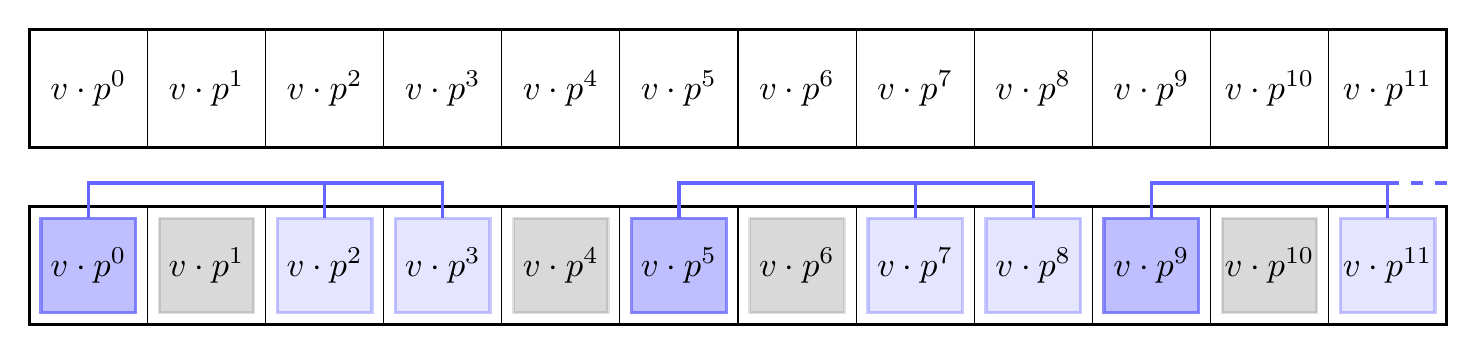
\begin{tikzpicture}[scale=1.5, every node/.style={scale=1.25}]
\begin{scope}[xshift=-0.5cm,yshift=-0.5cm]
\foreach \j in {0,...,1} {
\fill[white!100,yshift=\j*1.5cm] (0,0) -- (12, 0) -- (12, 1) -- (0, 1) -- cycle;
\draw[yshift=\j*1.5cm] (0,0) grid (12, 1);
\draw[very thick] (0,1.5*\j) -- (12, 1.5*\j) -- (12, 1.5*\j+1) -- (0, 1.5*\j+1) -- cycle;
}

\thickdotshape{blue!25}{blue!60}{0}{0*1.5}{0.75}
\thickdotshape{black!15}{black!60}{1}{0*1.5}{0.2}
\thickdotshape{blue!10}{blue!60}{2}{0*1.5}{0.35}
\thickdotshape{blue!10}{blue!60}{3}{0*1.5}{0.35}

\draw[very thick, blue!60] (0.5, 0*1.5+1-\lborder) -- (0.5, 0*1.5+1+2*\lborder) -- (2.5, 0*1.5+1+2*\lborder) -- (2.5, 0*1.5+1-\lborder);
\draw[very thick, blue!60] (2.5, 0*1.5+1+2*\lborder) -- (3.5, 0*1.5+1+2*\lborder) -- (3.5, 0*1.5+1-\lborder);

\thickdotshape{black!15}{black!60}{4}{0*1.5}{0.2}

\thickdotshape{blue!25}{blue!60}{5}{0*1.5}{0.75}
\thickdotshape{black!15}{black!60}{6}{0*1.5}{0.2}
\thickdotshape{blue!10}{blue!60}{7}{0*1.5}{0.35}
\thickdotshape{blue!10}{blue!60}{8}{0*1.5}{0.35}

\draw[very thick, blue!60] (5.5, 0*1.5+1-\lborder) -- (5.5, 0*1.5+1+2*\lborder) -- (7.5, 0*1.5+1+2*\lborder) -- (7.5, 0*1.5+1-\lborder);
\draw[very thick, blue!60] (7.5, 0*1.5+1+2*\lborder) -- (8.5, 0*1.5+1+2*\lborder) -- (8.5, 0*1.5+1-\lborder);

\thickdotshape{blue!25}{blue!60}{9}{0*1.5}{0.75}
\thickdotshape{black!15}{black!60}{10}{0*1.5}{0.2}
\thickdotshape{blue!10}{blue!60}{11}{0*1.5}{0.35}

\draw[very thick, blue!60] (9.5, 0*1.5+1-\lborder) -- (9.5, 0*1.5+1+2*\lborder) -- (11.5, 0*1.5+1+2*\lborder) -- (11.5, 0*1.5+1-\lborder);
\draw[very thick, blue!60] (11.5, 0*1.5+1+2*\lborder) -- (11.6, 0*1.5+1+2*\lborder);
\draw[very thick, blue!60] (11.7, 0*1.5+1+2*\lborder) -- (11.8, 0*1.5+1+2*\lborder);
\draw[very thick, blue!60] (11.9, 0*1.5+1+2*\lborder) -- (12, 0*1.5+1+2*\lborder);

\end{scope}
\foreach \i in {0,1,...,11} {
\foreach \j in {0,...,1} {
\node at (\i, 1.5*\j) {$v \cdot p^{\i}$};
}
}
\end{tikzpicture}
\end{center}

\newpage

\begin{center}
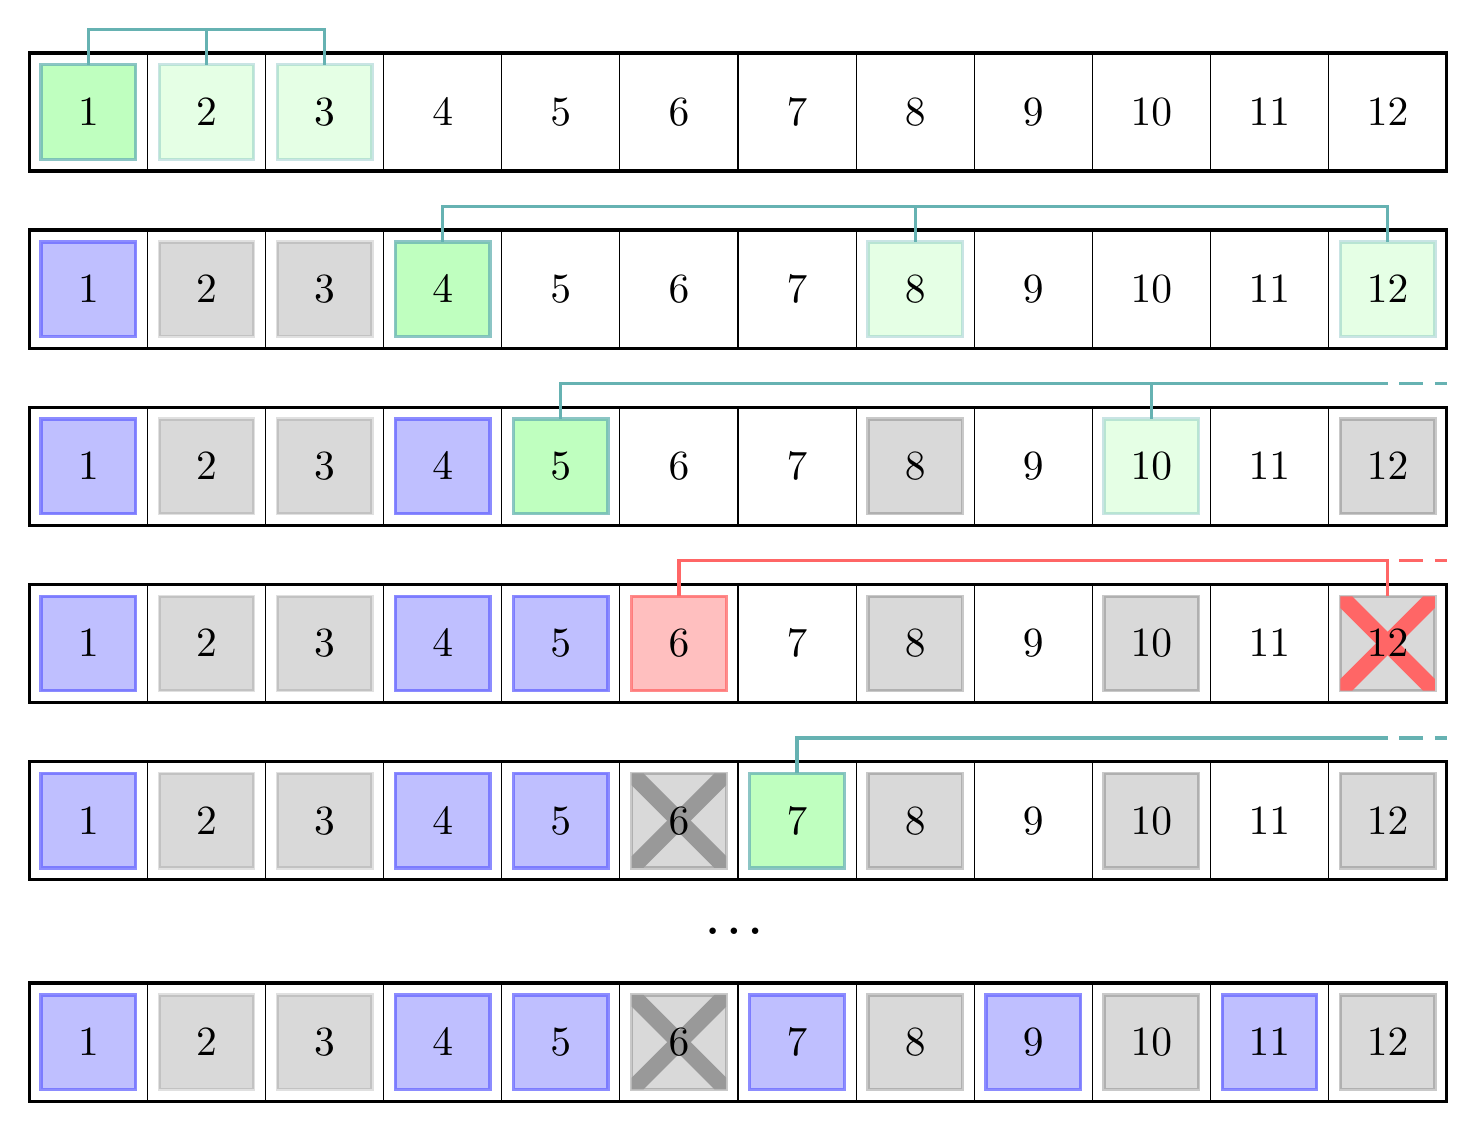
\begin{tikzpicture}[scale=1.5, every node/.style={scale=1.5}]
\begin{scope}[xshift=-0.5cm,yshift=-0.5cm]
\foreach \j in {-0.25,1,2,...,5} {
\fill[white!100,yshift=\j*1.5cm] (0,0) -- (12, 0) -- (12, 1) -- (0, 1) -- cycle;
\draw[yshift=\j*1.5cm] (0,0) grid (12, 1);
\draw[very thick] (0,1.5*\j) -- (12, 1.5*\j) -- (12, 1.5*\j+1) -- (0, 1.5*\j+1) -- cycle;
}
\thickdotshape{green!25}{teal!60}{0}{5*1.5}{0.75}
\thickdotshape{green!10}{teal!60}{1}{5*1.5}{0.35}
\thickdotshape{green!10}{teal!60}{2}{5*1.5}{0.35}
\draw[very thick, teal!60] (0+0.5,5*1.5+1-\lborder) -- (0+0.5,5*1.5+1+2*\lborder) -- (1+0.5, 5*1.5+1+2*\lborder) -- (1+0.5, 5*1.5+1-\lborder);
\draw[very thick, teal!60] (1+0.5, 5*1.5+1+2*\lborder) -- (2+0.5, 5*1.5+1+2*\lborder) -- (2+0.5, 5*1.5+1-\lborder);

\thickdotshape{blue!25}{blue!60}{0}{4*1.5}{0.75}
\thickdotshape{black!15}{black!60}{1}{4*1.5}{0.2}
\thickdotshape{black!15}{black!60}{2}{4*1.5}{0.2}
\thickdotshape{green!25}{teal!60}{3}{4*1.5}{0.75}
\thickdotshape{green!10}{teal!60}{7}{4*1.5}{0.35}
\thickdotshape{green!10}{teal!60}{11}{4*1.5}{0.35}
\draw[very thick, teal!60] (3+0.5,4*1.5+1-\lborder) -- (3+0.5,4*1.5+1+2*\lborder) -- (7+0.5, 4*1.5+1+2*\lborder) -- (7+0.5, 4*1.5+1-\lborder);
\draw[very thick, teal!60] (7+0.5, 4*1.5+1+2*\lborder) -- (11+0.5, 4*1.5+1+2*\lborder) -- (11+0.5, 4*1.5+1-\lborder);

\thickdotshape{blue!25}{blue!60}{0}{3*1.5}{0.75}
\thickdotshape{black!15}{black!60}{1}{3*1.5}{0.2}
\thickdotshape{black!15}{black!60}{2}{3*1.5}{0.2}
\thickdotshape{blue!25}{blue!60}{3}{3*1.5}{0.75}
\thickdotshape{black!15}{black!60}{7}{3*1.5}{0.35}
\thickdotshape{black!15}{black!60}{11}{3*1.5}{0.35}
\thickdotshape{green!25}{teal!60}{4}{3*1.5}{0.75}
\thickdotshape{green!10}{teal!60}{9}{3*1.5}{0.35}
\draw[very thick, teal!60] (4+0.5,3*1.5+1-\lborder) -- (4+0.5,3*1.5+1+2*\lborder) -- (9+0.5, 3*1.5+1+2*\lborder) -- (9+0.5, 3*1.5+1-\lborder);
\draw[very thick, teal!60] (9+0.5, 3*1.5+1+2*\lborder) -- (11.5, 3*1.5+1+2*\lborder);
\draw[very thick, teal!60] (11.6, 3*1.5+1+2*\lborder) -- (11.8, 3*1.5+1+2*\lborder);
\draw[very thick, teal!60] (11.9, 3*1.5+1+2*\lborder) -- (12, 3*1.5+1+2*\lborder);

\thickdotshape{blue!25}{blue!60}{0}{2*1.5}{0.75}
\thickdotshape{black!15}{black!60}{1}{2*1.5}{0.2}
\thickdotshape{black!15}{black!60}{2}{2*1.5}{0.2}
\thickdotshape{blue!25}{blue!60}{3}{2*1.5}{0.75}
\thickdotshape{black!15}{black!60}{7}{2*1.5}{0.35}
\thickdotshape{black!15}{black!60}{11}{2*1.5}{0.35}
\thickdotshape{blue!25}{blue!60}{4}{2*1.5}{0.75}
\thickdotshape{black!15}{black!60}{9}{2*1.5}{0.35}
\thickdotshape{red!25}{red!60}{5}{2*1.5}{0.75}
\xshape{red!60}{11}{2*1.5}
\draw[very thick, red!60] (5+0.5,2*1.5+1-\lborder) -- (5+0.5,2*1.5+1+2*\lborder) -- (11+0.5, 2*1.5+1+2*\lborder) -- (11+0.5, 2*1.5+1-\lborder);
\draw[very thick, red!60] (11.6, 2*1.5+1+2*\lborder) -- (11.8, 2*1.5+1+2*\lborder);
\draw[very thick, red!60] (11.9, 2*1.5+1+2*\lborder) -- (12, 2*1.5+1+2*\lborder);

\thickdotshape{blue!25}{blue!60}{0}{1*1.5}{0.75}
\thickdotshape{black!15}{black!60}{1}{1*1.5}{0.2}
\thickdotshape{black!15}{black!60}{2}{1*1.5}{0.2}
\thickdotshape{blue!25}{blue!60}{3}{1*1.5}{0.75}
\thickdotshape{black!15}{black!60}{7}{1*1.5}{0.35}
\thickdotshape{black!15}{black!60}{11}{1*1.5}{0.35}
\thickdotshape{blue!25}{blue!60}{4}{1*1.5}{0.75}
\thickdotshape{black!15}{black!60}{9}{1*1.5}{0.35}
\thickdotshape{black!15}{black!60}{5}{1*1.5}{0.35}
\xshape{black!40}{5}{1*1.5}
\thickdotshape{green!25}{teal!60}{6}{1*1.5}{0.75}
\draw[very thick, teal!60] (6+0.5,1*1.5+1-\lborder) -- (6+0.5,1*1.5+1+2*\lborder) -- (11.5, 1*1.5+1+2*\lborder);
\draw[very thick, teal!60] (11.6, 1*1.5+1+2*\lborder) -- (11.8, 1*1.5+1+2*\lborder);
\draw[very thick, teal!60] (11.9, 1*1.5+1+2*\lborder) -- (12, 1*1.5+1+2*\lborder);

\node at (6, 1.0625) {\textbf\ldots};

\thickdotshape{blue!25}{blue!60}{0}{-0.25*1.5}{0.75}
\thickdotshape{black!15}{black!60}{1}{-0.25*1.5}{0.2}
\thickdotshape{black!15}{black!60}{2}{-0.25*1.5}{0.2}
\thickdotshape{blue!25}{blue!60}{3}{-0.25*1.5}{0.75}
\thickdotshape{black!15}{black!60}{7}{-0.25*1.5}{0.35}
\thickdotshape{black!15}{black!60}{11}{-0.25*1.5}{0.35}
\thickdotshape{blue!25}{blue!60}{4}{-0.25*1.5}{0.75}
\thickdotshape{black!15}{black!60}{9}{-0.25*1.5}{0.35}
\thickdotshape{black!15}{black!60}{5}{-0.25*1.5}{0.35}
\xshape{black!40}{5}{-0.25*1.5}
\thickdotshape{blue!25}{blue!60}{6}{-0.25*1.5}{0.75}
\thickdotshape{blue!25}{blue!60}{8}{-0.25*1.5}{0.75}
\thickdotshape{blue!25}{blue!60}{10}{-0.25*1.5}{0.75}

\end{scope}
\foreach \i in {1,2,...,12} {
\foreach \j in {-0.25,1,2,...,5} {
\node at (\i-1, 1.5*\j) {\i};
}
}
\end{tikzpicture}
\end{center}
\end{document}
